\documentclass[a4paper, 12pt]{article}

% --- GÓI CẦN THIẾT ---
\usepackage[utf8]{inputenc}
\usepackage[T5]{fontenc}
\usepackage[vietnamese,english]{babel}

% --- Bố cục trang ---
\usepackage[
  a4paper,
  top=2.5cm,
  bottom=2.5cm,
  left=2.5cm,
  right=2.5cm,
  headheight=15pt,
  headsep=1cm
]{geometry}

% --- Hình ảnh và Bảng biểu ---
\usepackage{graphicx}
\usepackage{array}
\usepackage{tabularx}
\usepackage{longtable}
\usepackage{float}
\usepackage{booktabs}

% --- Định dạng văn bản và tiêu đề ---
\usepackage{titlesec}
\usepackage{indentfirst}
\usepackage{ragged2e}
\usepackage{setspace}
\onehalfspacing

% --- Toán học ---
\usepackage{amsmath, amssymb}

% --- Trích dẫn và Siêu liên kết ---
\usepackage{cite}
\usepackage[unicode,colorlinks=true, linkcolor=black, urlcolor=black, citecolor=black]{hyperref}

% --- TÙY CHỈNH TIÊU ĐỀ ---
\titleformat{\part}[display]
  {\normalfont\huge\bfseries\centering}
  {}
  {0pt}
  {\vspace{-2.5em}}
\titlespacing*{\part}{0pt}{*4}{*2}

\titleformat{\section}{\normalfont\Large\bfseries}{\thesection}{1em}{}
\titleformat{\subsection}{\normalfont\large\bfseries}{\thesubsection}{1em}{}
\titleformat{\subsubsection}{\normalfont\normalsize\bfseries}{\thesubsubsection}{1em}{}

\renewcommand{\contentsname}{\centering\huge\bfseries MỤC LỤC}
\setlength{\parskip}{0.45em}

\begin{document}

\begin{titlepage}
\bfseries
    \centering
    {\large {HỌC VIỆN CÔNG NGHỆ BƯU CHÍNH VIỄN THÔNG}}\\[0.5cm]
    {\large {KHOA CÔNG NGHỆ THÔNG TIN 1}}\\[0.5cm]
    \rule{3.5cm}{0.4pt}~\textbf{o0o}~\rule{3.5cm}{0.4pt}\\[1cm]
    
\includegraphics[width=0.22\textwidth]{Logo_PTIT_University.png}\\[1cm]

    {\LARGE {BÁO CÁO TỔNG KẾT THỰC TẬP CƠ SỞ}}\\[0.8cm]
    {\large {Đề tài: Observability-Aware Causal Neural Operators}}\\[0.2cm]
    {\large {for Probabilistic Full-Field Forecasting from Sparse Boundary Sensors}}\\[1cm]

    {\large LỚP: D23CQCE01-B} \\[0.2cm]

\begin{center}
\begin{tabular}{l l}
\large Vũ Hùng Anh & MSSV: B23DCDT022 \\
\end{tabular}
\end{center}

    \vspace{0.6cm}
    {\large Giảng viên hướng dẫn: TS. Nguyễn Tất Thắng} \\
    \vfill
    {\large HÀ NỘI, 04/2026}
\end{titlepage}

\newpage
\thispagestyle{empty}
\vspace*{-1cm}
\begin{center}
    {\Large\textbf{LỜI MỞ ĐẦU}}
\end{center}
\vspace{1cm}

\noindent
Trong quá trình thực hiện học phần Thực tập Cơ sở, em đã nghiên cứu bài toán học toán tử cho mô phỏng và dự báo trường mực nước biển trong điều kiện quan trắc thưa. Trọng tâm cuối cùng của đề tài là xây dựng một mô hình dự báo toàn trường từ một số ít cảm biến biên, đồng thời ước lượng được độ bất định của dự báo.

\vspace{1em}
\noindent
Em xin gửi lời cảm ơn chân thành tới thầy \textbf{TS. Nguyễn Tất Thắng} đã hướng dẫn, góp ý và định hướng để em hoàn thiện dần từ mô hình DeepONet ban đầu, qua các bước kiểm thử dữ liệu, chuyển sang dự báo nhân quả, và cuối cùng phát triển khung \textbf{Observability-Aware Variational Causal Neural Operator} (OVCNO).

\vspace{1em}
\noindent
Báo cáo này tổng hợp quá trình làm việc qua các tuần, kết quả chính của bài báo cuối cùng, các đóng góp kỹ thuật, kết quả thực nghiệm, hạn chế còn tồn tại và hướng phát triển tiếp theo. Do thời gian và dữ liệu còn giới hạn, báo cáo khó tránh khỏi thiếu sót; em mong nhận được góp ý của thầy để tiếp tục hoàn thiện nghiên cứu.

\vspace*{2em}
\begin{flushright}
    \textbf{Sinh viên thực hiện} \\[1em]
    Vũ Hùng Anh
\end{flushright}
\newpage

\vspace*{-1cm}
\begin{center}
    {\Large\textbf{MỤC LỤC}}
\end{center}
\vspace{0.5cm}
\renewcommand{\contentsname}{}
\tableofcontents
\newpage

\begin{center}
{\huge\bfseries Phần 1: Tổng quan đề tài và quá trình phát triển}
\end{center}
\addcontentsline{toc}{part}{Phần 1: Tổng quan đề tài và quá trình phát triển}

\section*{I. Bối cảnh và mục tiêu nghiên cứu}
\addcontentsline{toc}{section}{I. Bối cảnh và mục tiêu nghiên cứu}

Bài toán dự báo trường vật lý toàn miền từ quan trắc thưa có ý nghĩa quan trọng trong mô phỏng thủy động lực, dự báo ven bờ và thiết kế mạng cảm biến. Với khu vực Vịnh Bắc Bộ, trong khi trường mực nước biển là một đại lượng không gian--thời gian liên tục, dữ liệu quan trắc thực tế thường chỉ tồn tại tại một số ít trạm ven bờ hoặc điểm biên. Điều này dẫn đến một bài toán khó: từ lịch sử đo tại một số cảm biến biên, cần dự báo trường mực nước trong toàn miền ở các thời điểm tương lai.

Mục tiêu ban đầu của đề tài là học toán tử nghiệm của hệ phương trình nước nông bằng DeepONet. Tuy nhiên, qua quá trình thực nghiệm, đề tài được tái định vị từ bài toán \textit{reconstruction} sang bài toán \textit{causal forecasting}: mô hình chỉ được sử dụng dữ liệu quá khứ tại cảm biến và phải dự báo trường tương lai. Ở giai đoạn cuối, nghiên cứu tập trung vào câu hỏi:

\begin{quote}
\textit{Làm thế nào dự báo toàn trường từ cảm biến biên thưa trong khi vẫn biết vùng nào đáng tin cậy và vùng nào có độ bất định cao?}
\end{quote}

\section*{II. Tóm tắt tiến trình theo các giai đoạn}
\addcontentsline{toc}{section}{II. Tóm tắt tiến trình theo các giai đoạn}

\begin{longtable}{p{2.4cm} p{4.2cm} p{7.2cm}}
\toprule
\textbf{Giai đoạn} & \textbf{Trọng tâm} & \textbf{Kết quả chính} \\
\midrule
Tuần 3--4 & DeepONet 2D cho Vịnh Bắc Bộ & Xây dựng pipeline dữ liệu, solver Godunov HLL, mô hình DeepONet ban đầu; đạt Rel-L2 khoảng 21.5\% trên case Vịnh Bắc Bộ. \\
Tuần 5--6 & Physics-informed và phân tích lỗi & Thử PI-DeepONet, anomaly shift, heatmap, time-series, spatial error và spectral analysis; nhận diện hạn chế của pipeline dữ liệu. \\
Tuần 7--8 & Partial observation & So sánh full-state, interior sensors và boundary sensors trên PDEBench; chứng minh học toán tử từ quan trắc thưa có tính khả thi. \\
Tuần 9 & Debug hệ thống & Sửa lỗi C-property, tidal forcing, sensor placement, ocean-only label; cải thiện Fourier DeepONet từ Rel-L2 93.6\% xuống 14.8\%. \\
Tuần 10 & Causal forecasting & Chuyển từ reconstruction sang ForecastDeepONet với LSTM causal branch; chỉ sử dụng quá khứ tại cảm biến. \\
Tuần 11 & Variational Causal Operator & Bổ sung latent stochastic state và uncertainty head; chuyển từ dự báo điểm sang dự báo phân phối. \\
Giai đoạn cuối & OVCNO và paper & Phát triển OVCNO với sensor geometry encoder và learned observability proxy; hoàn thiện paper và đánh giá trên PDEBench, Copernicus SSH. \\
\bottomrule
\end{longtable}

\begin{center}
{\huge\bfseries Phần 2: Phương pháp đề xuất OVCNO}
\end{center}
\addcontentsline{toc}{part}{Phần 2: Phương pháp đề xuất OVCNO}

\section*{I. Phát biểu bài toán}
\addcontentsline{toc}{section}{I. Phát biểu bài toán}

Cho miền không gian $\Omega \subset \mathbb{R}^2$ và trường mục tiêu $\eta(x,y,t)$, chỉ có $K$ cảm biến trên biên miền với lịch sử đo:
\begin{equation}
S_{0:T_{\mathrm{obs}}} = \{S(t)\}_{t=0}^{T_{\mathrm{obs}}}, \qquad S(t)=[s_1(t),\ldots,s_K(t)].
\end{equation}
Mục tiêu là dự báo trường tương lai:
\begin{equation}
\eta(x,y,t), \qquad (x,y)\in\Omega,\quad t>T_{\mathrm{obs}}.
\end{equation}
Do $K \ll N_xN_y$ và các cảm biến nằm trên biên, bài toán này là một bài toán nghịch đảo dưới quan sát thiếu. Vì vậy, mô hình không chỉ cần dự báo giá trị trung bình mà còn cần dự báo độ bất định.

\section*{II. Kiến trúc OVCNO}
\addcontentsline{toc}{section}{II. Kiến trúc OVCNO}

Mô hình cuối cùng được đề xuất là \textbf{Observability-Aware Variational Causal Neural Operator} (OVCNO). Kiến trúc bao gồm bốn thành phần chính:

\begin{itemize}
    \item \textbf{Sensor geometry encoder:} mã hóa đồng thời giá trị đo và tọa độ cảm biến, giúp mô hình hiểu cảm biến nằm ở đâu.
    \item \textbf{Set encoder:} tổng hợp tập cảm biến theo cách bất biến hoán vị, hỗ trợ số lượng cảm biến thay đổi.
    \item \textbf{Causal temporal encoder:} dùng LSTM để xử lý lịch sử quá khứ, đảm bảo không nhìn vào tương lai.
    \item \textbf{Variational latent state và observability proxy:} biểu diễn nhiều trạng thái nội miền khả dĩ và học một điểm số $o_\psi(x,y,t)$ mô tả mức độ vị trí truy vấn được ràng buộc bởi mạng cảm biến.
\end{itemize}

\begin{figure}[H]
    \centering
    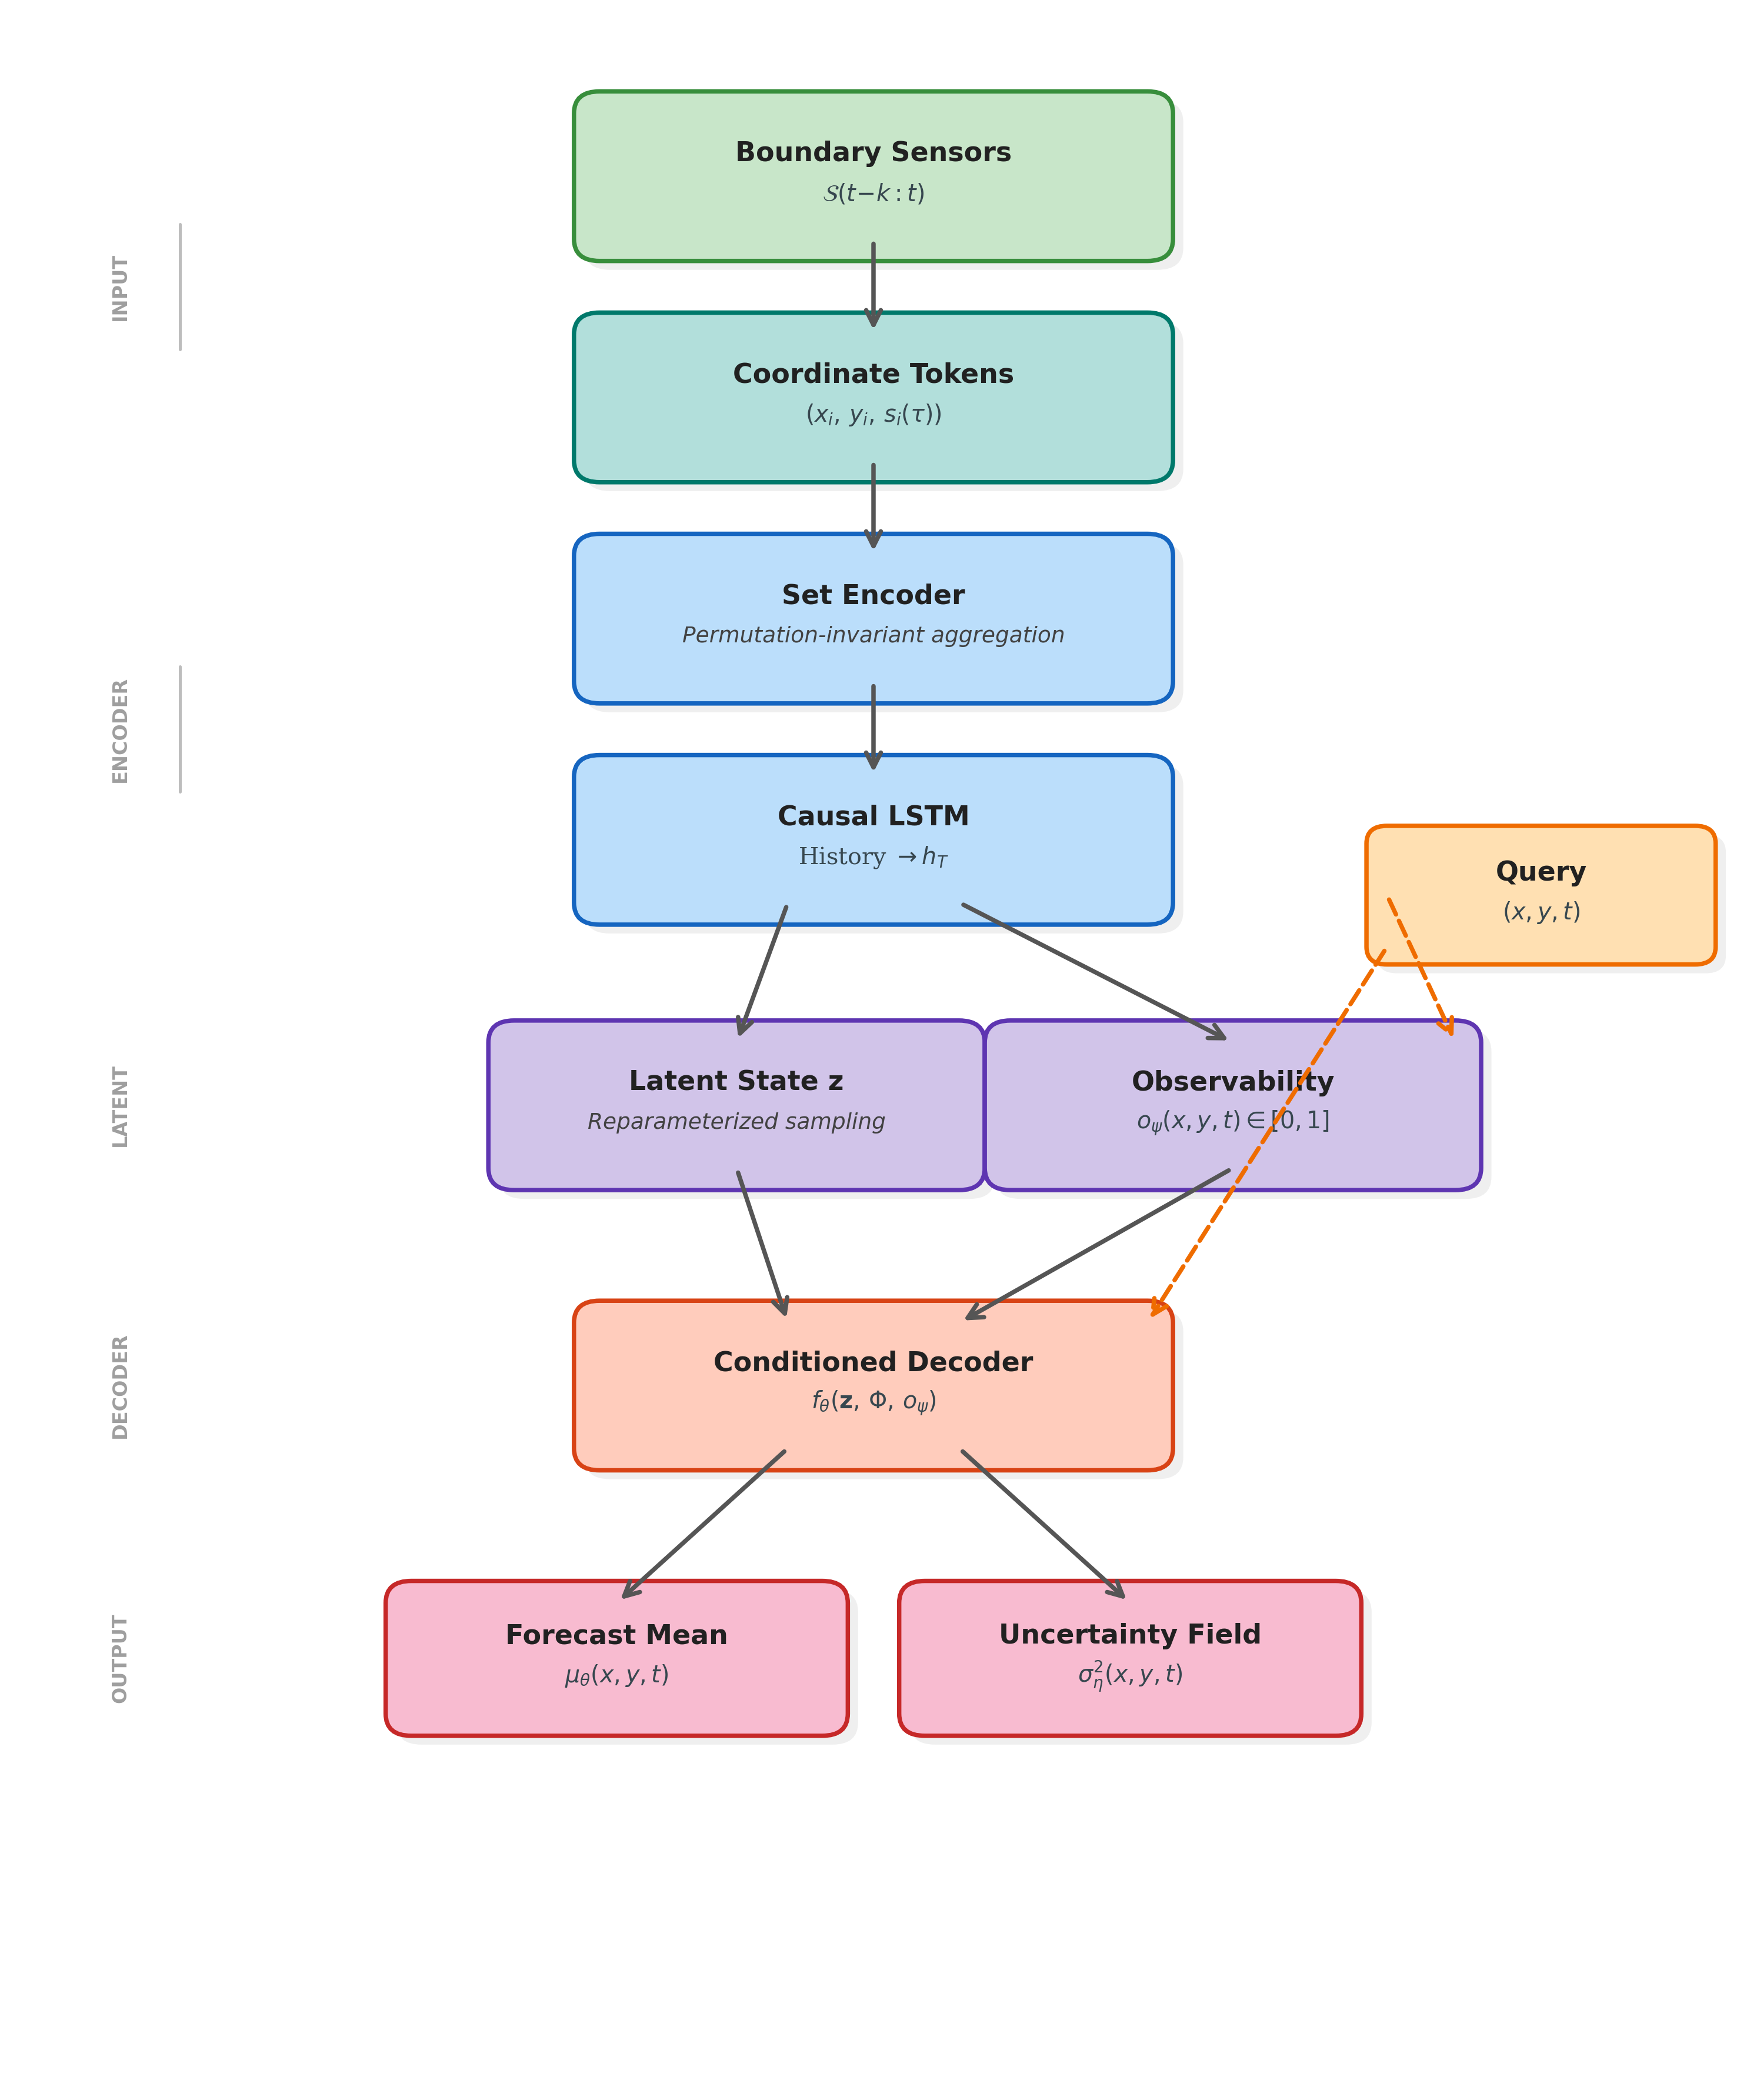
\includegraphics[width=0.88\textwidth]{../docs/figures/ovcno_architecture.png}
    \caption{Sơ đồ tổng quan kiến trúc OVCNO.}
\end{figure}

Đầu ra của mô hình là phân phối Gaussian theo từng điểm truy vấn:
\begin{equation}
p_\theta(\eta(x,y,t)\mid S_{0:T_{\mathrm{obs}}}) =
\mathcal{N}(\mu_\theta(x,y,t), \sigma_\theta^2(x,y,t)).
\end{equation}
Nhờ đó, mô hình có thể đánh giá không chỉ dự báo trung bình mà còn cả khoảng tin cậy và rủi ro dự báo.

\begin{center}
{\huge\bfseries Phần 3: Thực nghiệm và kết quả}
\end{center}
\addcontentsline{toc}{part}{Phần 3: Thực nghiệm và kết quả}

\section*{I. Benchmark kiểm soát: PDEBench}
\addcontentsline{toc}{section}{I. Benchmark kiểm soát: PDEBench}

PDEBench được sử dụng như một benchmark kiểm soát với các trajectory mô phỏng độc lập. Dữ liệu được chia theo chỉ số simulation, nên các trajectory held-out tách biệt với trajectory huấn luyện. Bài toán sparse-boundary được xây dựng bằng cách giữ lại 16 cảm biến trên biên và dự báo toàn trường.

\begin{table}[H]
\centering
\caption{Kết quả chính trên PDEBench 2D SWE.}
\resizebox{\textwidth}{!}{
\begin{tabular}{lccccc}
\toprule
\textbf{Mô hình} & \textbf{Input} & \textbf{Rel-L2 (\%)} & \textbf{RMSE} & \textbf{NLL} & \textbf{Cov@95\%} \\
\midrule
U-Net 2D & Dense/full state & $\sim$12.80 & -- & -- & -- \\
FNO-2D & Dense/full state & 5.13 & -- & -- & -- \\
Deterministic Causal Operator & 16 boundary sensors & 4.46 & 0.0125 & -- & -- \\
VCO & 16 boundary sensors & 4.42 & 0.0121 & -3.12 & 94.80\% \\
\textbf{OVCNO} & \textbf{16 boundary sensors} & \textbf{4.38} & \textbf{0.0118} & \textbf{-3.25} & \textbf{95.20\%} \\
\bottomrule
\end{tabular}}
\end{table}

Kết quả cho thấy OVCNO giữ được chất lượng dự báo điểm tương đương các baseline sparse-boundary, đồng thời cải thiện NLL và coverage. Đây là kiểm chứng quan trọng rằng việc thêm latent stochastic state và observability proxy không làm suy giảm đáng kể khả năng dự báo.

\section*{II. Applied OSSE: Copernicus SSH Vịnh Bắc Bộ}
\addcontentsline{toc}{section}{II. Applied OSSE: Copernicus SSH Vịnh Bắc Bộ}

Thí nghiệm ứng dụng sử dụng sản phẩm SSH từ Copernicus Marine Service trong tháng 1/2024 trên miền Vịnh Bắc Bộ. Dữ liệu gồm lưới $73 \times 61$, độ phân giải thời gian 1 giờ. Do chỉ có một tháng dữ liệu, kết quả được diễn giải là \textbf{held-out chronological validation OSSE}, không phải final operational test.

\begin{table}[H]
\centering
\caption{Kết quả trên Copernicus SSH Gulf of Tonkin.}
\resizebox{\textwidth}{!}{
\begin{tabular}{lccccccc}
\toprule
\textbf{Mô hình} & \textbf{RMSE} & \textbf{MAE} & \textbf{NLL} & \textbf{CRPS} & \textbf{Avg.W} & \textbf{Cov@95\%} & \textbf{Corr}$_S$ \\
\midrule
Optimal Interpolation & 0.1140 & 0.0890 & -- & -- & -- & -- & -- \\
Persistence & 0.0820 & 0.0610 & -- & -- & -- & -- & -- \\
Deterministic Causal Op. & 0.0680 & 0.0482 & -- & -- & -- & -- & -- \\
VCO & 0.0765 & 0.0564 & -1.92 & 0.043 & \textbf{0.209} & 79.7\% & 0.446 \\
\textbf{OVCNO} & \textbf{0.0683} & \textbf{0.0505} & \textbf{-2.39} & \textbf{0.036} & 0.287 & \textbf{94.8\%} & \textbf{0.523} \\
\bottomrule
\end{tabular}}
\end{table}

OVCNO cải thiện rõ rệt các metric xác suất: NLL giảm từ -1.92 xuống -2.39, CRPS giảm từ 0.043 xuống 0.036, coverage tăng từ 79.7\% lên 94.8\%. Đổi lại, khoảng dự báo rộng hơn (Avg.W 0.287 so với 0.209), thể hiện trade-off giữa calibration và sharpness.

\section*{III. Phân tích theo forecast horizon}
\addcontentsline{toc}{section}{III. Phân tích theo forecast horizon}

\begin{table}[H]
\centering
\caption{Horizon-conditioned evaluation trên Copernicus SSH.}
\begin{tabular}{lcccc}
\toprule
\textbf{Model} & \textbf{Lead time} & \textbf{RMSE} & \textbf{Avg.W} & \textbf{Cov@95\%} \\
\midrule
VCO & +1h & 0.044 & 0.164 & 84.3\% \\
VCO & +24h & 0.102 & 0.252 & 77.3\% \\
\textbf{OVCNO} & \textbf{+1h} & \textbf{0.039} & 0.172 & \textbf{93.2\%} \\
\textbf{OVCNO} & \textbf{+24h} & \textbf{0.090} & 0.314 & \textbf{94.7\%} \\
\bottomrule
\end{tabular}
\end{table}

Kết quả theo horizon cho thấy khi dự báo xa hơn, sai số và độ rộng khoảng dự báo đều tăng. Tuy nhiên, OVCNO duy trì coverage gần mức danh nghĩa 95\% từ +1h tới +24h, trong khi VCO có xu hướng under-cover ngày càng mạnh.

\section*{IV. Phân tích định tính và observability}
\addcontentsline{toc}{section}{IV. Phân tích định tính và observability}

\begin{figure}[H]
    \centering
    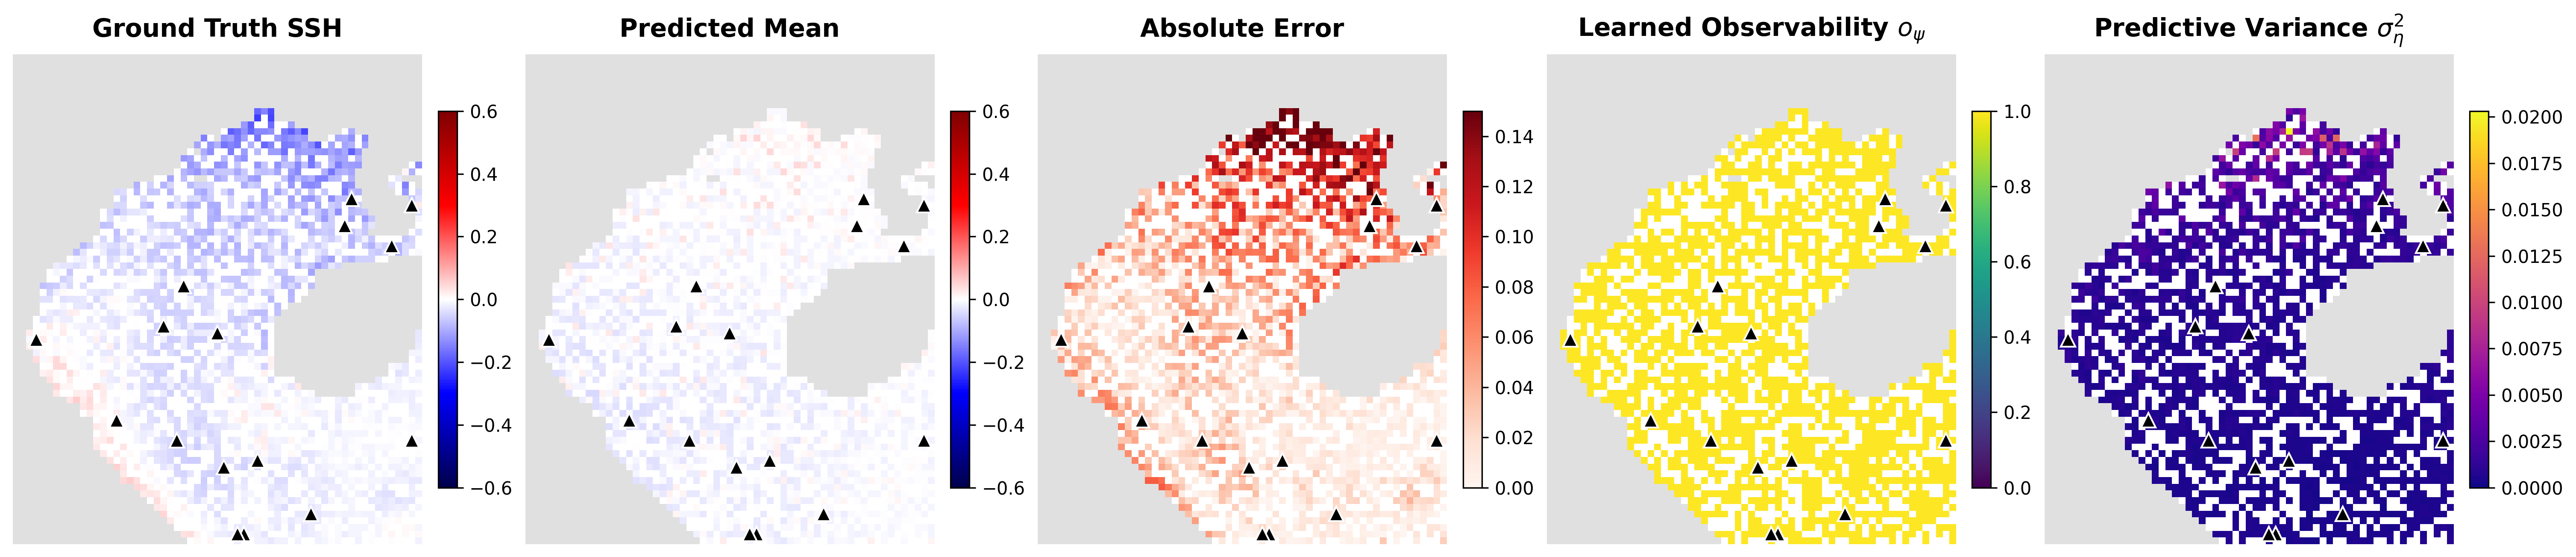
\includegraphics[width=\textwidth]{../docs/figures/observability_maps.png}
    \caption{Bản đồ dự báo, sai số, observability proxy và phương sai dự báo.}
\end{figure}

Các bản đồ định tính cho thấy vùng có observability score cao thường tương ứng với sai số thấp hơn và phương sai dự báo nhỏ hơn. Điều này ủng hộ cách diễn giải $o_\psi$ như một proxy học được cho mức độ vị trí truy vấn được ràng buộc bởi cảm biến.

\begin{figure}[H]
    \centering
    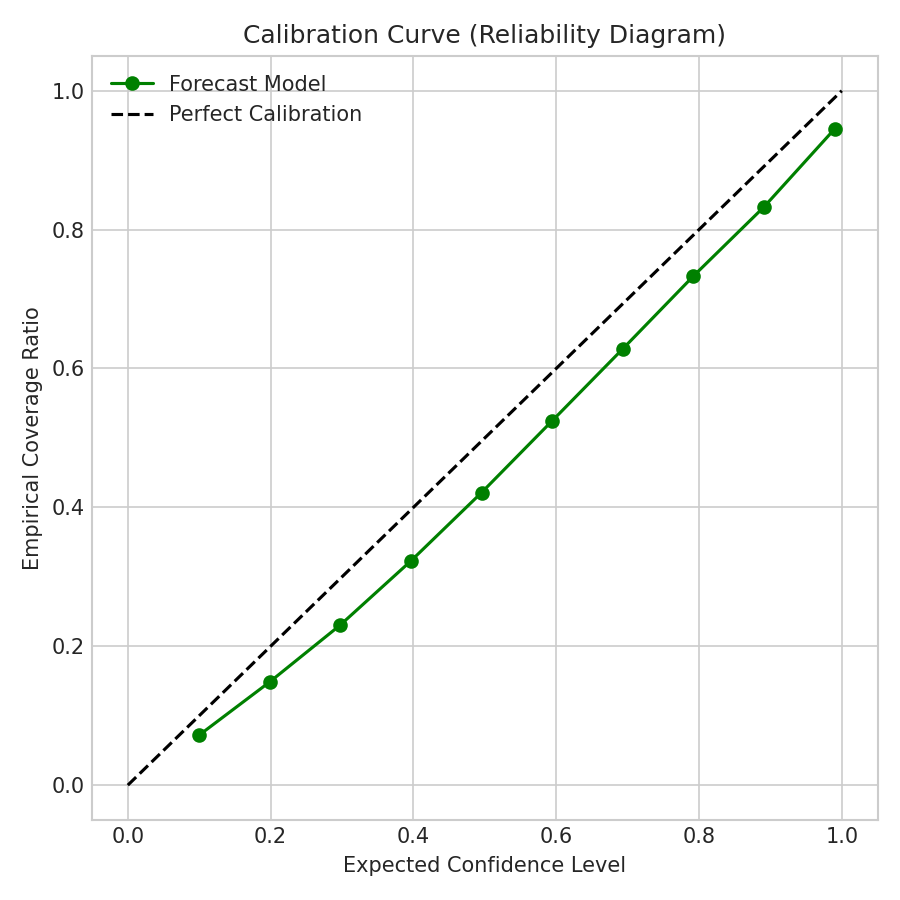
\includegraphics[width=0.82\textwidth]{../docs/figures/calibration_curve.png}
    \caption{Phân tích calibration của dự báo xác suất.}
\end{figure}

\section*{V. Real-station geometry OSSE}
\addcontentsline{toc}{section}{V. Real-station geometry OSSE}

Ngoài sensor biên đều, đề tài đánh giá thêm bố trí 12 trạm thực tế tại khu vực Vịnh Bắc Bộ. Đây là Level-1 OSSE: tọa độ trạm lấy từ nguồn thực tế, còn giá trị sensor được sample từ sản phẩm gridded ocean analysis.

\begin{figure}[H]
    \centering
    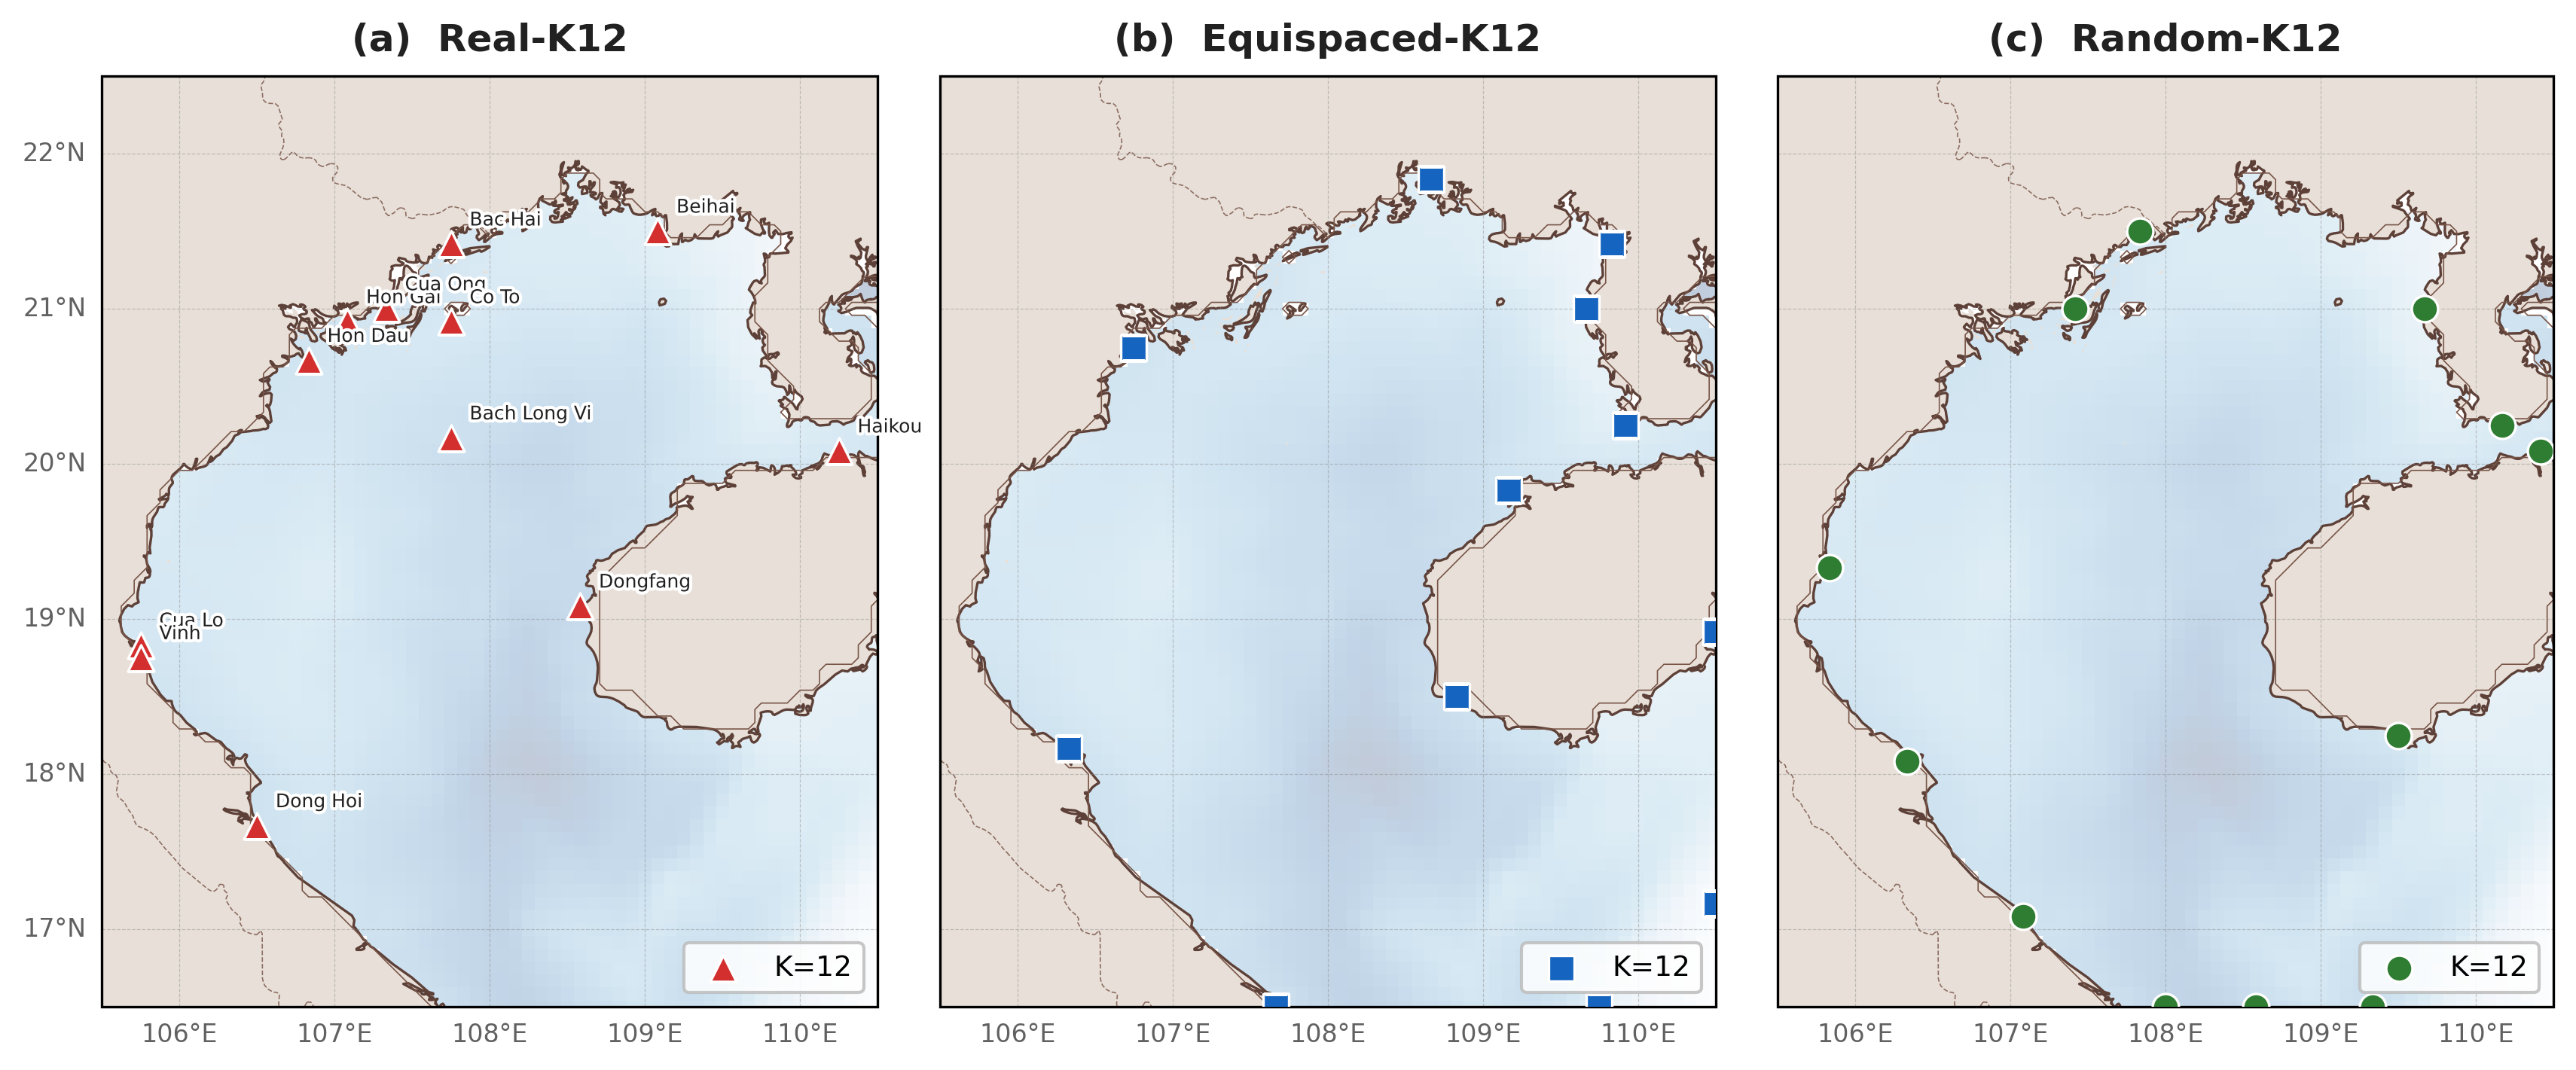
\includegraphics[width=0.95\textwidth]{../docs/figures/layout_comparison.png}
    \caption{So sánh ba bố trí cảm biến trong thí nghiệm real-station geometry OSSE: Real-K12, Equispaced-K12 và Random-K12.}
\end{figure}

\begin{table}[H]
\centering
\caption{Ảnh hưởng của bố trí cảm biến tại budget $K=12$.}
\begin{tabular}{lccc}
\toprule
\textbf{Layout} & \textbf{RMSE} & \textbf{CRPS} & \textbf{Cov@95\%} \\
\midrule
Real-K12 & $0.083 \pm 0.017$ & $0.044 \pm 0.006$ & $94.2 \pm 2.1\%$ \\
Equispaced-K12 & $0.076 \pm 0.011$ & $0.042 \pm 0.004$ & $93.6 \pm 1.7\%$ \\
Random-K12 & $0.070 \pm 0.001$ & $0.039 \pm 0.000$ & $94.0 \pm 0.2\%$ \\
\bottomrule
\end{tabular}
\end{table}

Kết quả cho thấy ở budget $K=12$, training-seed variance lớn hơn layout variance, nên chưa thể kết luận một layout có ưu thế tuyệt đối về point accuracy. Tuy nhiên, real-station geometry thể hiện độ ổn định tốt hơn khi có sensor dropout, cho thấy topology có ý nghĩa đối với robustness vận hành.

\begin{figure}[H]
    \centering
    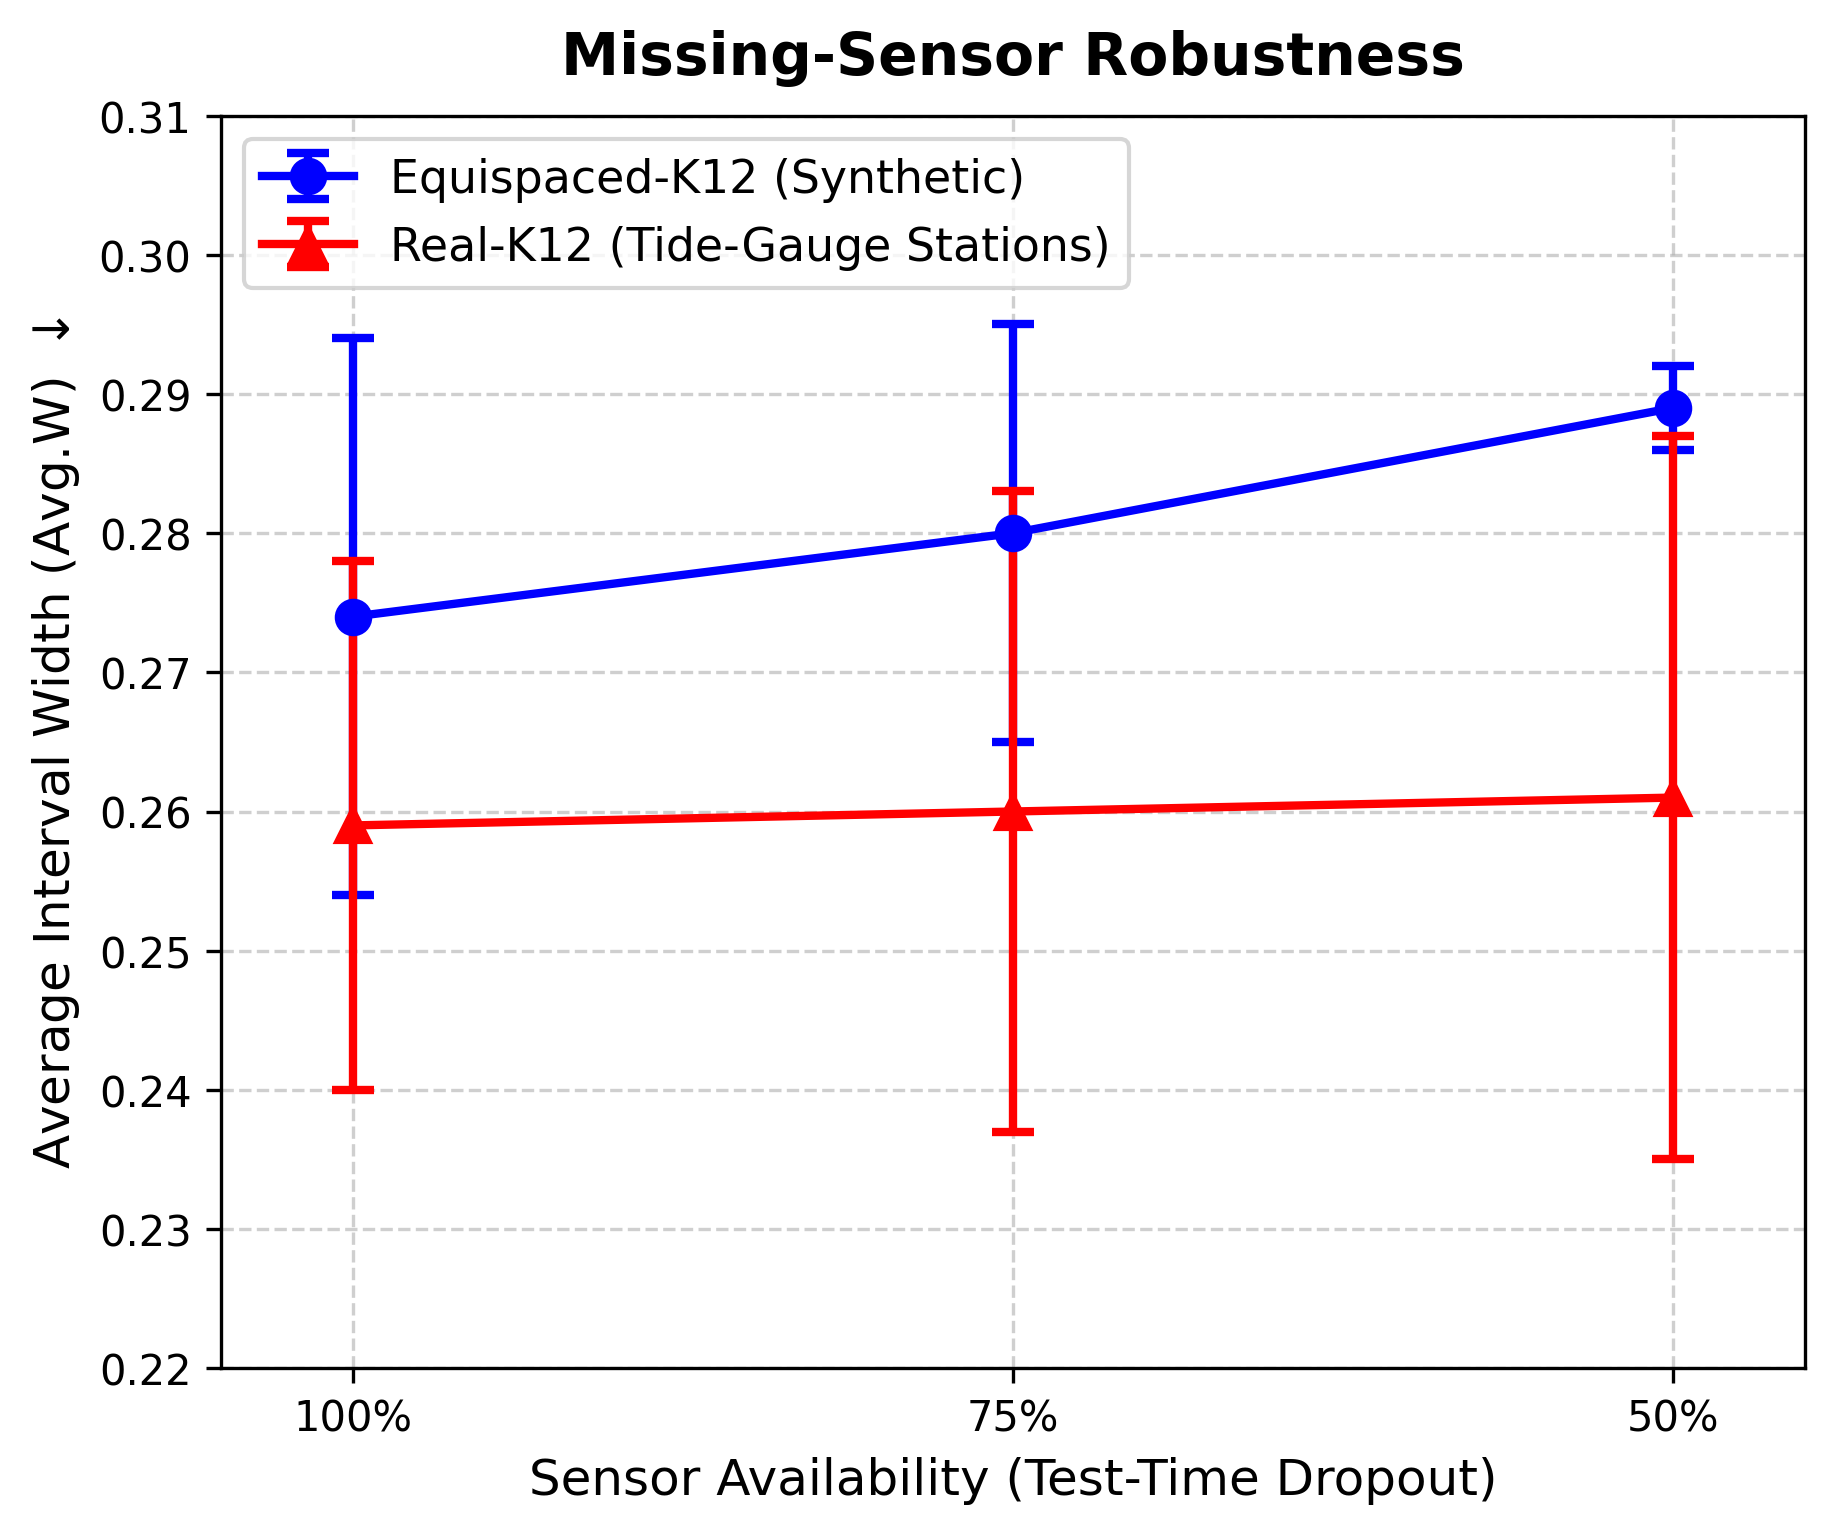
\includegraphics[width=0.78\textwidth]{../docs/figures/robustness_curve.png}
    \caption{Robustness dưới test-time sensor dropout.}
\end{figure}

\clearpage
\begin{center}
{\huge\bfseries Phần 4: Đóng góp, hạn chế và hướng phát triển}
\end{center}
\addcontentsline{toc}{part}{Phần 4: Đóng góp, hạn chế và hướng phát triển}

\section*{I. Đóng góp chính}
\addcontentsline{toc}{section}{I. Đóng góp chính}

Đề tài đạt được các đóng góp chính sau:
\begin{enumerate}
    \item Tái định vị bài toán từ reconstruction sang causal sparse-boundary forecasting, phù hợp hơn với điều kiện vận hành thực tế.
    \item Xây dựng OVCNO, một neural operator xác suất kết hợp sensor geometry, causal encoding, variational latent state và learned observability proxy.
    \item Chứng minh trên PDEBench rằng mô hình giữ được độ chính xác dự báo điểm trong controlled held-out trajectory benchmark.
    \item Chứng minh trên Copernicus SSH rằng OVCNO cải thiện mạnh về calibration, NLL, CRPS và error--uncertainty alignment so với VCO.
    \item Đánh giá real-station geometry OSSE, chỉ ra vai trò của topology trong robustness dưới sensor dropout.
\end{enumerate}

\section*{II. Hạn chế}
\addcontentsline{toc}{section}{II. Hạn chế}

Một số hạn chế còn tồn tại:
\begin{itemize}
    \item \textbf{Copernicus chỉ là validation OSSE:} dữ liệu hiện tại chỉ gồm một tháng, chưa có final operational test độc lập.
    \item \textbf{Observability proxy chưa phải observability hình thức:} $o_\psi$ là proxy học từ dữ liệu, không phải rank condition trong control theory.
    \item \textbf{Calibration--sharpness trade-off:} OVCNO đạt coverage tốt hơn nhưng interval rộng hơn VCO.
    \item \textbf{Training stability:} thí nghiệm real-station cho thấy seed variance còn lớn.
    \item \textbf{Cross-product robustness:} thử nghiệm HYCOM cho thấy có thể xuất hiện mean--variance coupling artifact khi đổi sản phẩm dữ liệu.
\end{itemize}

\section*{III. Hướng phát triển tiếp theo}
\addcontentsline{toc}{section}{III. Hướng phát triển tiếp theo}

Các hướng phát triển tự nhiên gồm:
\begin{itemize}
    \item Mở rộng dữ liệu Copernicus/HYCOM nhiều tháng hoặc nhiều mùa để có bộ train, validation và test độc lập.
    \item Tích hợp quan trắc tide-gauge thật và xử lý datum alignment để chuyển từ Level-1 sang Level-2 OSSE.
    \item Thiết kế kiến trúc decoupled mean--variance, trong đó observability chỉ điều tiết variance pathway.
    \item Thêm conformal calibration hoặc post-hoc recalibration để giảm interval width mà vẫn giữ coverage.
    \item Đánh giá dài hạn với autoregressive rollouts và network sensor dropout thực tế.
\end{itemize}

\section*{IV. Kết luận}
\addcontentsline{toc}{section}{IV. Kết luận}

Báo cáo tổng kết này trình bày quá trình phát triển từ DeepONet mô phỏng thủy triều ban đầu tới OVCNO cho dự báo xác suất toàn trường từ cảm biến biên thưa. Kết quả cuối cùng cho thấy hướng tiếp cận observability-aware có giá trị rõ ràng trong bài toán sparse coastal sensing: mô hình không chỉ dự báo trường tương lai mà còn cung cấp thông tin về độ tin cậy không gian của dự báo.

Mặc dù vẫn còn các giới hạn về dữ liệu, test split và độ ổn định huấn luyện, đề tài đã hình thành được một pipeline nghiên cứu hoàn chỉnh gồm phát biểu bài toán, mô hình, benchmark kiểm soát, case study ứng dụng, phân tích bất định, phân tích sensor geometry và định hướng phát triển tiếp theo.

\begin{thebibliography}{9}
\bibitem{deeponet}
L. Lu, P. Jin, G. Pang, Z. Zhang, and G. E. Karniadakis,
``Learning nonlinear operators via DeepONet based on the universal approximation theorem of operators,''
\textit{Nature Machine Intelligence}, 2021.

\bibitem{fno}
Z. Li et al.,
``Fourier Neural Operator for Parametric Partial Differential Equations,''
\textit{International Conference on Learning Representations}, 2021.

\bibitem{pdebench}
M. Takamoto et al.,
``PDEBench: An Extensive Benchmark for Scientific Machine Learning,''
\textit{NeurIPS Datasets and Benchmarks}, 2022.

\bibitem{vae}
D. P. Kingma and M. Welling,
``Auto-Encoding Variational Bayes,''
\textit{International Conference on Learning Representations}, 2014.

\bibitem{cmems}
J.-M. Lellouche et al.,
``Recent updates to the Copernicus Marine Service global ocean monitoring and forecasting system,''
\textit{Ocean Science}, 2018.
\end{thebibliography}

\end{document}
